\section*{Goldponsor}
\begin{flushright}
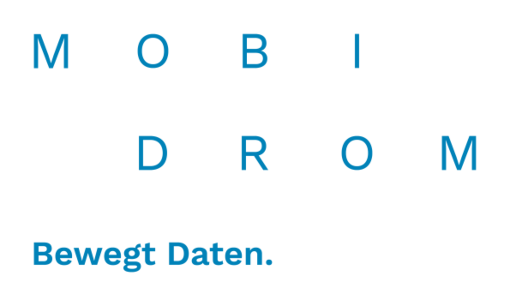
\includegraphics[width=1.0\textwidth]{104_Mobidrom_Logo.png}
\end{flushright}
\noindent
Die {\bfseries NRW.Mobidrom GmbH} ist eine Gesellschaft des Landes NRW und fungiert seit der Gründung im Juli 2023 als Ansprechpartner und Umsetzungseinheit für digitalisierte und vernetzte Mobilität. Zentrale Aufgabe des Mobidroms ist die flächendeckende, verkehrsträgerübergreifende und diskriminierungsfreie Bereitstellung von Mobilitätsdaten über die Mobidrom Datenplattform (derzeit in Entwicklung).

\noindent
Das Mobidrom steht allen Datengebern und -nutzern im Bereich Mobilitätsdaten beratend zur Seite und beteiligt sich aktiv an Entwicklung und Betrieb von Open-Source-Anwendungen im Mobilitätsbereich. Dies umfasst derzeit vor allem die Entwicklung eines Routing-Dienstes, der bestehende Projekte verkehrsträgerübergreifend integriert. Darüber hinaus verantwortet das Mobidrom die Weiterentwicklung und den Betrieb des reichweitenstarken Verkehrsportals Verkehr.NRW, welches Nutzern Daten und Dienste des Mobidroms zugänglich macht und die Reiseplanung ermöglicht. Webseite: www.mobidrom.nrw


